% Source: http://tex.stackexchange.com/a/149780/23931
\documentclass[tikz]{standalone}
\usetikzlibrary{calc}
\begin{document}
\pagecolor{gray}
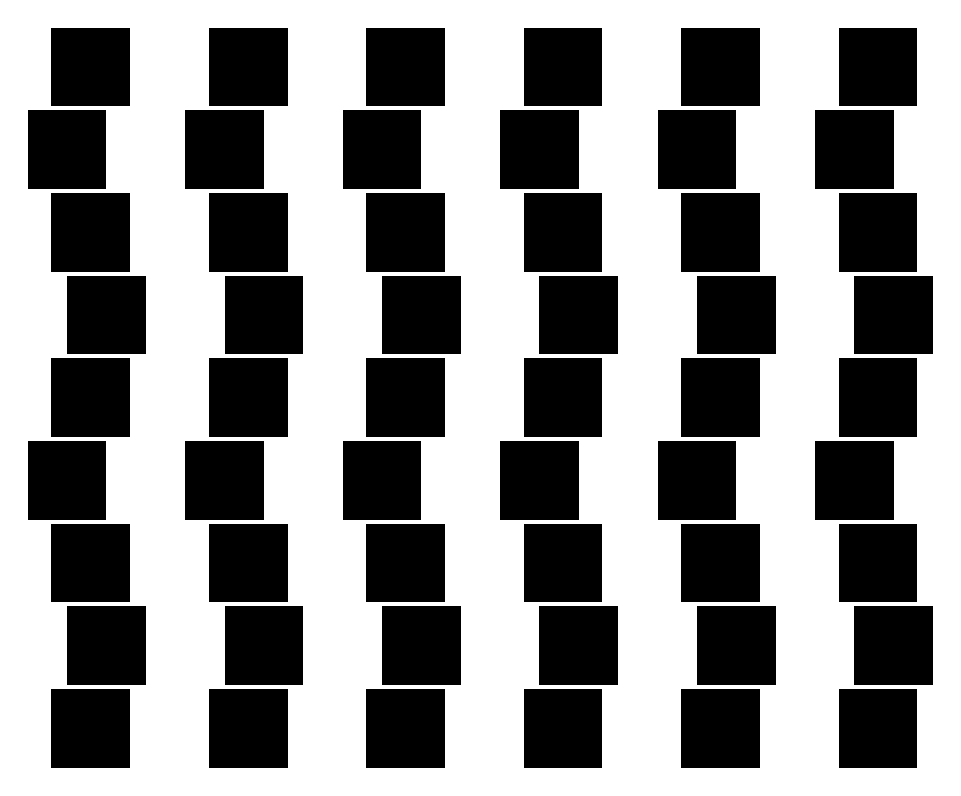
\begin{tikzpicture}
    \pgfmathsetmacro{\offsety}{.05};
    \foreach \y / \offsetx in {0/0.3,1/0.5,2/0.3,3/0,4/0.3,5/0.5,6/0.3,7/0,8/0.3}
    \foreach \x in {0,...,10}{%
            \pgfmathifthenelse{mod(\x,2) == 0}{"black"}{"white"}
            %\ifodd\x \def\squarecolor{white} \else \def\squarecolor{black} \fi %Other way, use \squarecolor inside fill options
            \fill[\pgfmathresult] ($(\x,\y)+(\offsetx,\offsety*\y)$) rectangle +(1,1);
        }
\end{tikzpicture}
\end{document}